% Options for packages loaded elsewhere
\PassOptionsToPackage{unicode}{hyperref}
\PassOptionsToPackage{hyphens}{url}
%
\documentclass[
]{book}
\usepackage{lmodern}
\usepackage{amssymb,amsmath}
\usepackage{ifxetex,ifluatex}
\ifnum 0\ifxetex 1\fi\ifluatex 1\fi=0 % if pdftex
  \usepackage[T1]{fontenc}
  \usepackage[utf8]{inputenc}
  \usepackage{textcomp} % provide euro and other symbols
\else % if luatex or xetex
  \usepackage{unicode-math}
  \defaultfontfeatures{Scale=MatchLowercase}
  \defaultfontfeatures[\rmfamily]{Ligatures=TeX,Scale=1}
\fi
% Use upquote if available, for straight quotes in verbatim environments
\IfFileExists{upquote.sty}{\usepackage{upquote}}{}
\IfFileExists{microtype.sty}{% use microtype if available
  \usepackage[]{microtype}
  \UseMicrotypeSet[protrusion]{basicmath} % disable protrusion for tt fonts
}{}
\makeatletter
\@ifundefined{KOMAClassName}{% if non-KOMA class
  \IfFileExists{parskip.sty}{%
    \usepackage{parskip}
  }{% else
    \setlength{\parindent}{0pt}
    \setlength{\parskip}{6pt plus 2pt minus 1pt}}
}{% if KOMA class
  \KOMAoptions{parskip=half}}
\makeatother
\usepackage{xcolor}
\IfFileExists{xurl.sty}{\usepackage{xurl}}{} % add URL line breaks if available
\IfFileExists{bookmark.sty}{\usepackage{bookmark}}{\usepackage{hyperref}}
\hypersetup{
  pdftitle={My First Bookdown},
  pdfauthor={Kaeli Mueller},
  hidelinks,
  pdfcreator={LaTeX via pandoc}}
\urlstyle{same} % disable monospaced font for URLs
\usepackage{color}
\usepackage{fancyvrb}
\newcommand{\VerbBar}{|}
\newcommand{\VERB}{\Verb[commandchars=\\\{\}]}
\DefineVerbatimEnvironment{Highlighting}{Verbatim}{commandchars=\\\{\}}
% Add ',fontsize=\small' for more characters per line
\usepackage{framed}
\definecolor{shadecolor}{RGB}{248,248,248}
\newenvironment{Shaded}{\begin{snugshade}}{\end{snugshade}}
\newcommand{\AlertTok}[1]{\textcolor[rgb]{0.94,0.16,0.16}{#1}}
\newcommand{\AnnotationTok}[1]{\textcolor[rgb]{0.56,0.35,0.01}{\textbf{\textit{#1}}}}
\newcommand{\AttributeTok}[1]{\textcolor[rgb]{0.77,0.63,0.00}{#1}}
\newcommand{\BaseNTok}[1]{\textcolor[rgb]{0.00,0.00,0.81}{#1}}
\newcommand{\BuiltInTok}[1]{#1}
\newcommand{\CharTok}[1]{\textcolor[rgb]{0.31,0.60,0.02}{#1}}
\newcommand{\CommentTok}[1]{\textcolor[rgb]{0.56,0.35,0.01}{\textit{#1}}}
\newcommand{\CommentVarTok}[1]{\textcolor[rgb]{0.56,0.35,0.01}{\textbf{\textit{#1}}}}
\newcommand{\ConstantTok}[1]{\textcolor[rgb]{0.00,0.00,0.00}{#1}}
\newcommand{\ControlFlowTok}[1]{\textcolor[rgb]{0.13,0.29,0.53}{\textbf{#1}}}
\newcommand{\DataTypeTok}[1]{\textcolor[rgb]{0.13,0.29,0.53}{#1}}
\newcommand{\DecValTok}[1]{\textcolor[rgb]{0.00,0.00,0.81}{#1}}
\newcommand{\DocumentationTok}[1]{\textcolor[rgb]{0.56,0.35,0.01}{\textbf{\textit{#1}}}}
\newcommand{\ErrorTok}[1]{\textcolor[rgb]{0.64,0.00,0.00}{\textbf{#1}}}
\newcommand{\ExtensionTok}[1]{#1}
\newcommand{\FloatTok}[1]{\textcolor[rgb]{0.00,0.00,0.81}{#1}}
\newcommand{\FunctionTok}[1]{\textcolor[rgb]{0.00,0.00,0.00}{#1}}
\newcommand{\ImportTok}[1]{#1}
\newcommand{\InformationTok}[1]{\textcolor[rgb]{0.56,0.35,0.01}{\textbf{\textit{#1}}}}
\newcommand{\KeywordTok}[1]{\textcolor[rgb]{0.13,0.29,0.53}{\textbf{#1}}}
\newcommand{\NormalTok}[1]{#1}
\newcommand{\OperatorTok}[1]{\textcolor[rgb]{0.81,0.36,0.00}{\textbf{#1}}}
\newcommand{\OtherTok}[1]{\textcolor[rgb]{0.56,0.35,0.01}{#1}}
\newcommand{\PreprocessorTok}[1]{\textcolor[rgb]{0.56,0.35,0.01}{\textit{#1}}}
\newcommand{\RegionMarkerTok}[1]{#1}
\newcommand{\SpecialCharTok}[1]{\textcolor[rgb]{0.00,0.00,0.00}{#1}}
\newcommand{\SpecialStringTok}[1]{\textcolor[rgb]{0.31,0.60,0.02}{#1}}
\newcommand{\StringTok}[1]{\textcolor[rgb]{0.31,0.60,0.02}{#1}}
\newcommand{\VariableTok}[1]{\textcolor[rgb]{0.00,0.00,0.00}{#1}}
\newcommand{\VerbatimStringTok}[1]{\textcolor[rgb]{0.31,0.60,0.02}{#1}}
\newcommand{\WarningTok}[1]{\textcolor[rgb]{0.56,0.35,0.01}{\textbf{\textit{#1}}}}
\usepackage{longtable,booktabs}
% Correct order of tables after \paragraph or \subparagraph
\usepackage{etoolbox}
\makeatletter
\patchcmd\longtable{\par}{\if@noskipsec\mbox{}\fi\par}{}{}
\makeatother
% Allow footnotes in longtable head/foot
\IfFileExists{footnotehyper.sty}{\usepackage{footnotehyper}}{\usepackage{footnote}}
\makesavenoteenv{longtable}
\usepackage{graphicx,grffile}
\makeatletter
\def\maxwidth{\ifdim\Gin@nat@width>\linewidth\linewidth\else\Gin@nat@width\fi}
\def\maxheight{\ifdim\Gin@nat@height>\textheight\textheight\else\Gin@nat@height\fi}
\makeatother
% Scale images if necessary, so that they will not overflow the page
% margins by default, and it is still possible to overwrite the defaults
% using explicit options in \includegraphics[width, height, ...]{}
\setkeys{Gin}{width=\maxwidth,height=\maxheight,keepaspectratio}
% Set default figure placement to htbp
\makeatletter
\def\fps@figure{htbp}
\makeatother
\setlength{\emergencystretch}{3em} % prevent overfull lines
\providecommand{\tightlist}{%
  \setlength{\itemsep}{0pt}\setlength{\parskip}{0pt}}
\setcounter{secnumdepth}{5}
\usepackage{booktabs}
\usepackage[]{natbib}
\bibliographystyle{apalike}

\title{My First Bookdown}
\author{Kaeli Mueller}
\date{2021-03-04}

\begin{document}
\maketitle

{
\setcounter{tocdepth}{1}
\tableofcontents
}
\hypertarget{introduction}{%
\chapter{Introduction}\label{introduction}}

This example book will show how to use bookdown to put together digital books. We are going to use some work we did on the Palmer Penquins dataset for this project.

Chapter \ref{penguins} is about making some exploratory plots.

\hypertarget{penguins}{%
\chapter{Palmer Penguins}\label{penguins}}

\hypertarget{palmer-penguins}{%
\chapter{Palmer Penguins}\label{palmer-penguins}}

\hypertarget{subtitle}{%
\section{Subtitle}\label{subtitle}}

\hypertarget{subheading}{%
\subsection{Subheading}\label{subheading}}

Today we are going to work with the \textbf{Palmer Penguins} dataset from the \texttt{palmerpenguins}
package. Install the package as follows:

\begin{Shaded}
\begin{Highlighting}[]
\CommentTok{#Eval = False means that it does not get run every time the document is knitted}
\CommentTok{#echo = TRUE  means it shows up but that it is not evaluated}
\KeywordTok{install.packages}\NormalTok{(}\StringTok{"palmerpenguins"}\NormalTok{) }\CommentTok{# add a comment}
\end{Highlighting}
\end{Shaded}

\begin{figure}

{\centering 
\includegraphics[width=0.3\linewidth]{C:/Users/Kaeli/Documents/Computational_Methods/Bookdown_project/test/logo} 

}

\caption{Logo of the palmerpenguins R package}\label{fig:logo}
\end{figure}

We are writing this in R Markdown because you can do all sorts of things in
R Markdown, such as embedding code in text: 2 + 2 = 4
\#Shows up in your document as 2 + 2 = 4 because you but the ` around the code that you wanted to execute

\begin{Shaded}
\begin{Highlighting}[]
\CommentTok{#this runs the chunk but doesn't show the weird message every time you load it}
\KeywordTok{library}\NormalTok{(palmerpenguins)}
\end{Highlighting}
\end{Shaded}

\begin{verbatim}
## Warning: package 'palmerpenguins' was built under R version 4.0.4
\end{verbatim}

\begin{Shaded}
\begin{Highlighting}[]
\KeywordTok{library}\NormalTok{(tidyverse)}
\end{Highlighting}
\end{Shaded}

\begin{verbatim}
## Warning: package 'tibble' was built under R version 4.0.4
\end{verbatim}

\begin{verbatim}
## Warning: package 'tidyr' was built under R version 4.0.4
\end{verbatim}

\begin{verbatim}
## Warning: package 'dplyr' was built under R version 4.0.4
\end{verbatim}

\hypertarget{the-dataset}{%
\section{The dataset}\label{the-dataset}}

Let's take a look at the datasets available in the \texttt{palmerpenguins} package:

\begin{Shaded}
\begin{Highlighting}[]
\KeywordTok{head}\NormalTok{(penguins)}
\end{Highlighting}
\end{Shaded}

\begin{verbatim}
## # A tibble: 6 x 8
##   species island bill_length_mm bill_depth_mm flipper_length_~ body_mass_g sex  
##   <fct>   <fct>           <dbl>         <dbl>            <int>       <int> <fct>
## 1 Adelie  Torge~           39.1          18.7              181        3750 male 
## 2 Adelie  Torge~           39.5          17.4              186        3800 fema~
## 3 Adelie  Torge~           40.3          18                195        3250 fema~
## 4 Adelie  Torge~           NA            NA                 NA          NA <NA> 
## 5 Adelie  Torge~           36.7          19.3              193        3450 fema~
## 6 Adelie  Torge~           39.3          20.6              190        3650 male 
## # ... with 1 more variable: year <int>
\end{verbatim}

\begin{quote}
``Capturing and measuring penguins was a lot of fun!'' (Anonymous technician)
\#formatted in a different way so that it clearly looks like a quote
\end{quote}

\hypertarget{penguin-measurements}{%
\subsection{Penguin measurements}\label{penguin-measurements}}

\#This makes it into a bulletted list

The table \texttt{penguins} includes the following measurements:

\begin{enumerate}
\def\labelenumi{\arabic{enumi}.}
\tightlist
\item
  Bill length;
\item
  Bill depth;
\item
  Flipper length;
\item
  Body mass.
  \#a number 1 then a . signals that this is the beginning of a numbered list
  \#even if you put all 1's in the list in the knitted document they will show up correctly
\end{enumerate}

\hypertarget{relationship-between-flipper-length-and-bill-length-by-species}{%
\subsubsection{Relationship between flipper length and bill length by species}\label{relationship-between-flipper-length-and-bill-length-by-species}}

We are going to make a plot showing how flipper length and bill length vary in
different species of penguin:

\begin{figure}

{\centering 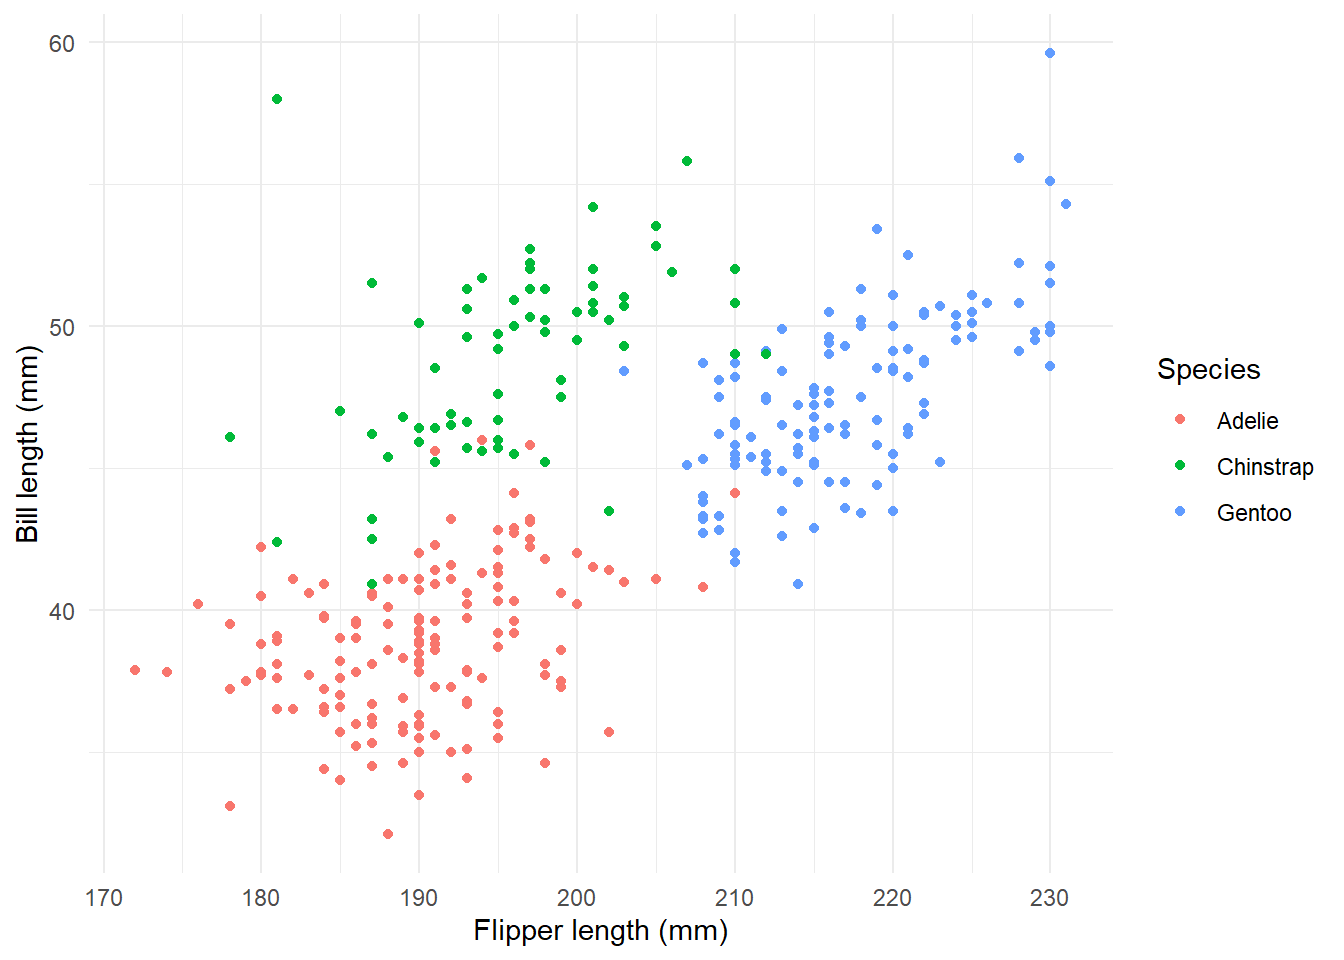
\includegraphics{test_files/figure-latex/plot-1} 

}

\caption{My plot}\label{fig:plot}
\end{figure}

For more information about the \texttt{palmerpenguins} package, visit \href{https://allisonhorst.github.io/palmerpenguins/}{their website}.
\#this is how you embed a link

This is a paragraph.

This is a new paragraph.

Referencing Figure \ref{fig:logo} and Figure \ref{fig:plot}

Building our own database:
-do it through R sql lite
-eval = false for the chunks that build the database and echo = true
-all chunks should have different names, unless they are unnamed

  \bibliography{book.bib,packages.bib}

\end{document}
